\documentclass[11pt,english,british]{report}
\usepackage[a4paper]{geometry}
%\usepackage[T1]{fontenc}
\usepackage[latin9]{inputenc}
\usepackage{setspace}
\geometry{verbose,tmargin=3cm,bmargin=3cm,lmargin=3.5cm,rmargin=2.4cm}
%\usepackage{fancyhdr}
%\pagestyle{fancy}
%\setcounter{secnumdepth}{3}
\usepackage[british]{babel}

\usepackage{amsmath}
\usepackage{amssymb}
\usepackage{cancel}
%\usepackage{gensymb}
\usepackage{graphicx}
\usepackage{esint}
\usepackage{mdsymbol}
\usepackage{esvect} 
%\usepackage{lipsum}
\usepackage{hhline}
\usepackage{eurosym}
\usepackage{listings}
\usepackage{booktabs}
\usepackage{amssymb}
\usepackage{mathrsfs}
\usepackage{commath}
\usepackage{adjustbox}
\usepackage{booktabs}
\usepackage{array}
\usepackage{lscape}
\usepackage[xspace]{ellipsis}
\usepackage{color}
\usepackage{float}
\usepackage{caption}
\usepackage{afterpage}

			\usepackage{titlesec}
			
			\titleformat{\chapter}[display]
			{\normalfont\huge\bfseries}{\chaptertitlename\ \thechapter}{20pt}{\Huge}
			
			% this alters "before" spacing (the second length argument) to 0
			\titlespacing*{\chapter}{0pt}{0pt}{32pt}
			
			\usepackage{etoolbox}
			\makeatletter
			\patchcmd{\chapter}{\if@openright\cleardoublepage\else\clearpage\fi}{}{}{}
			\makeatother
			
			\usepackage[unicode=true,pdfusetitle,
			bookmarks=true,bookmarksnumbered=false,bookmarksopen=false,
			breaklinks=true,pdfborder={0 0 0},backref=page,colorlinks=false]
			{hyperref}

\definecolor{mygreen}{rgb}{0,0.6,0}
\definecolor{mygray}{rgb}{0.5,0.5,0.5}
\definecolor{mymauve}{rgb}{0.58,0,0.82}

\begin{document}

\title{Placeholder Tex Doc}
\author{Conor Dooley}
\begin{titlepage}
	
%	\pagenumbering{gobble}
	
	\setstretch{1.25}
	
	\begin{spacing}{3}
		
		\noindent \begin{center}
			
			{\huge{}ADPLL Network on an FPGA}
			\par\end{center}{\huge \par}
	\end{spacing}
	
	\bigskip{}
	
	\begin{center}
		{\Large{}Conor Dooley}
	\end{center}
	
	\vspace{1.25cm}
	
	\begin{center}
		%
\includegraphics[width=0.15\paperwidth]{ucd_crest.pdf}\vspace{0.75cm}
		\includegraphics[width=0.2\paperwidth]{UCD_crest.pdf}\vspace{0.25cm}
	\end{center}
	
	
	\bigskip{}
	
	\begin{center}
		{\huge{}Masters Project Interim Report }
	\end{center}
	
	\vspace{1.cm}
	
	
	{\Large{}\bigskip{}
		\bigskip{}
	}{\Large \par}
	
	\noindent \begin{center}
		\begin{tabular}{lll}
			\textbf{\large{}Research Supervisors:} & \qquad{}\qquad{} & {\large{}Dr Elena Blokhina \& Brian Mulkeen}\\
		\end{tabular}
		
		\par\end{center}
	
	\vspace{1cm}
	\noindent \begin{center}
		{\large{}January  2019}
		\par\end{center}{\large \par}
	
\end{titlepage}
\setcounter{page}{1} 
\pagenumbering{roman}
\setstretch{1.05}

\addcontentsline{toc}{chapter}{\contentsname}

\tableofcontents{}

\pagebreak{}

%\begin{dedication}
%Dedicated to google and wikipedia  
%\end{dedication}

%\setcounter{page}{1} 
%\pagenumbering{roman}

%\addtocontents{toc}{\protect{\pdfbookmark[0]{Abstract}{toc}}}
%\pagestyle{empty}
%\addcontentsline{toc}{chapter}{Abstract}
%\phantomsection

\pagestyle{plain}

\setstretch{1.3}
\doublespacing
\pagenumbering{arabic}
\setcounter{page}{1} 
\chapter{Background Review}
\section{Brief Overview}
In a world where the demand for high performance hand-held computing devices continues to grow and the prevalence of ``smart'' devices is increasing, the problem of maintaining the steady gain in performance of Systems-On-Chip remains at the fore. %TODO cite?
The main drivers of performance in Systems-On-Chip are the number of transistors on a chip and the frequency at which it is clocked.
As the number of transistors on a chip has increased roughly following Moore's Law, the increase in clock frequency has not been able to follow a similar linear trajectory, having remained roughly equivalent for the last number of years \cite{ross2008cpu}.

This plateauing of clock frequency has been caused by high power consumption due to the demands placed by the global distribution of a high frequency clock, often the single biggest consumer of power on the chip \cite{tiwari1998reducing}.
In a world where low power devices are desirable, especially with the growing demand of the Internet-Of-Things where high power consumption goes directly against one of the key pillars of the technology. %TODO Pillars of what?

In digital systems, two main approaches are used when designing the clocking system. In both cases, the chip is broken down into small areas in which all transistors are clocked synchronously, with the size constrained by the ability to deliver a quality clock signal to all transistors. The first of these methods is Globally Synchronous Locally Synchronous, or GSLS, where all of these sub areas on the chip are synchronised with each other. In practice, however, this is very difficult to achieve, as extremely high precision is required across the entire area of the chip, and doing so leads to high power consumption.
In contrast in a Globally Asynchronous Locally Synchronous clock delivery system the ``local'' areas are not synchronised with other. This reduces the clocking system's complexity and thus the power consumption and chip area used, at the expense of communication speed between blocks. %TODO citation?
A GSLS, system, however has the advantages of deterministic behaviour and greater rates of communication between clocking areas and, as such, remains a desirable system design. A number of methods which deliver GSLS clocking exist at present such as clock trees as well as emerging technologies such as ADPLL networks.

\section{The Impact of Clocking Errors}
In Figure \ref{fig:eldar_why_precise_clocking} the data path between two synchronously clocked registers is shown, with the circuit's function being carried out by the combinatorial network between the registers.
Each register has a setup time, which represents the amount of time that the input value to a register must remain constant before the clock edge, and a hold time, the time for which the input must remain constant after a clock edge.
\begin{figure}[h]
	\centering
	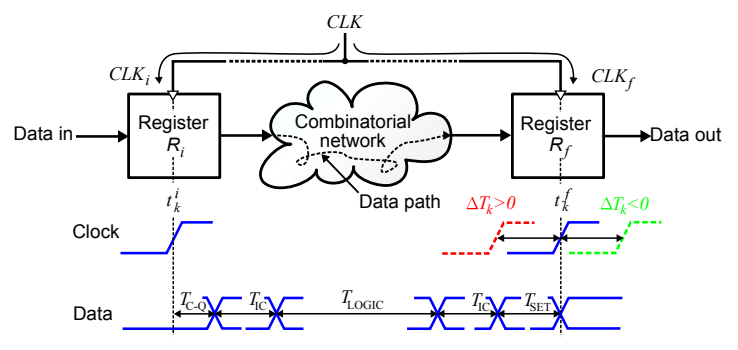
\includegraphics[scale=0.5]{../eldar_why_precise_clocking}
	\caption{Data Flow in a Clocked System \cite{zianbetov2013phd}.}
	\label{fig:eldar_why_precise_clocking}
\end{figure}\\

A lack of synchronisation between the clock edges will manifest itself as a time difference between the clocking events at both registers, $\Delta T = t^i_k - t^f_k$. $\Delta T$ is considered to be ergodic and can be described by an average deviation called skew and random process, normally modelled as a Gaussian random variable. If $\Delta T$ is negative this reduces the time available for the intervening combinatorial network thereby, having the same effect as a reduction in clocking frequency.
The most common sources of clock error are caused by mismatches which usually stem from production, such as differences in the length of clocking paths, buffer delays or in the parameters of either active or passive components in the clock distribution network. These all manifest themselves as skew, while the noise in active components will appear as jitter in the clock signal.

\section{Traditional Solutions}
A number of traditional solutions exist which provide GSLS clocking systems, using a variety of techniques. The most simple of these use the clock distribution network's symmetry in order to deliver the clock in phase, at all locations in the chip and are named according to their geometry with the main variants being branch-trees, X-trees or H-trees. 
\begin{figure}[h]
	\centering
	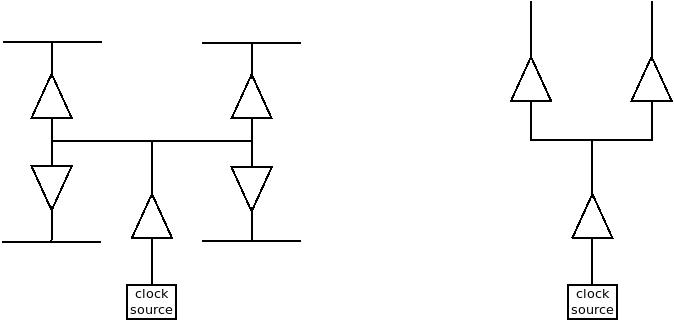
\includegraphics[scale=0.2]{../trees}
	\caption{H and Branch Tree Clock Distribution Systems.}
	\label{fig:trees}
\end{figure}

While on the surface these appear simple, the task of obtaining an exact matching is, in practice, the limiting factor in this design. Even if the clock distribution system is geometrically symmetrical, production mismatches in either active or passive components will lead to a skew that varies from part to part. In order to minimise the impact of production tolerances, the dimensions of components in the distribution network can be increased, thus reducing the relative variation possible. However this has the impact of increasing the power consumption of the distribution network \cite{tiwari1998reducing}.
Designs do exist in which the electrical lines used in the tree network are replaced by waveguides for optical signals, which negates the electrical losses, however, this technique suffers from being a newer technology and as such is expensive to realise \cite{haurylau2006chip}.

A mesh clock distribution network is an alternate design where the clock is delivered using a Cartesian grid of distribution lines and variation in skew is inversely proportional to the density of the grid. According to Abdelhadi \textit{et al} (2010) clock meshes ``\textit{achieve low and deterministic skew, low skew variations, and low jitter}'', all desirable characteristics for a clock distribution system. However they dissipate more power due to extra capacitive loading attributable to vast number of lines required to form the grid Similarly tree distribution networks suffer from potential mismatch in production and alleviation through increasing of distribution system dimensions will again lead to higher power consumption \cite{abdelhadi2010timing}. 
\begin{figure}[h]
	\centering
	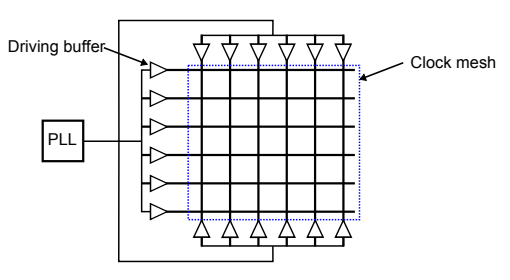
\includegraphics[scale=0.6]{eldar_mesh}
	\caption{Mesh Clock Distribution System \cite{zianbetov2013phd}.}
	\label{fig:mesh}
\end{figure}

In a tree type distribution system, skew due to the manufacturing process can be partly accounted for by means of a skew compensation system, of which there are two main types. These types are defined by the location of the control mechanism with those having one controller located at the clock source, known as ``centralised'' methods, and those with multiple controllers in the individual clocking areas known as ``decentralised''. In a centralised skew compensation circuit, the skew across the chip is calculated by the central controller which then manipulates the distribution network in order to deliver a more in-phase clock around the chip. This, however, adds complication to a circuit which already is a large consumer of power and as such increases the power usage.

As the name suggest a decentralised skew compensation technique delegates this responsibility to the individual clock regions. For example, Yamashita \textit{et al} (2005) designed a system in which each clocking area or ``leaf node'' contains a partial clock tree. Each of these ``leaves'' is able to compare its clock phase to the neighbouring node, and based on the result, tune an adjustable delay buffer \cite{yamashita2005dynamic}. While this method can compensate for process, voltage and temperature variation, it does not address the power consumption due to the delivery of a high frequency clock across the entire chip area.

\section{Multi-oscillator Designs}
The designs described previously, are all similar in that they have a single central oscillator that provides the clock for all areas of the chip, whereas the following methods attempt to synchronise multiple oscillators, each of which provides the clock for a single clocking area. The main advantage of a multi-oscillator design, is that as each clocking area has its clock created locally, there is no problem with signal degradation. Similar to a decentralised skew compensation scheme comparisons are only made to neighbouring blocks and as such there is reduced power loss due to transmission.
\begin{figure}[h]
	\centering
	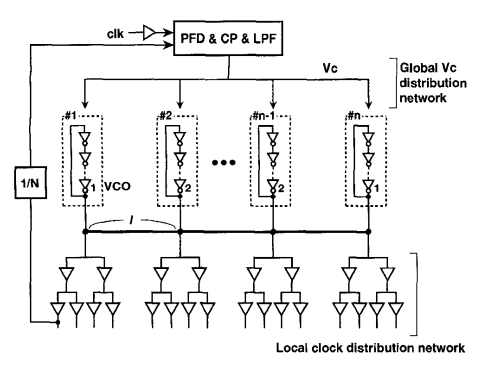
\includegraphics[scale=0.5]{../mizuno1998noise}
	\caption{Coupled Oscillator Clock Delivery Circuit \cite{mizuno1998noise}.}
	\label{fig:mizuno1998noise}
\end{figure}
One such method is a network of oscillators as in Figure \ref{fig:mizuno1998noise} which uses coupled PLLs to generate local clocks. The advantage of this method is that only the control voltage $v_c$ needs delivery to all areas of the chip, thus alleviating the need for a power hungry distribution circuit, while also being more noise-immune than the transmission of a high frequency clock. However this design still suffers from clock variation as all VCOs are fed the same control voltage, and this is acknowledged by the authors:
\begin{quotation}
	\singlespacing
	\textit{Unfortunately, as with the conventional ... method, distributing the VCOs over the entire chip causes the problem that jitter and skew are increased by variations in the fabrication process (static), temperature, and power supply (dynamic)} \cite{mizuno1998noise}.
	\doublespacing
\end{quotation}
This design also only compares the phase of a single branch of the distribution network with the reference, in order calculate the control voltage which again may contribute to a degradation in clock synchronisation. %TODO why

Another potential multi-oscillator design synchronises the oscillators using the phase relationship with the oscillators in the neighbouring clocking area. Once again, this negates the requirement for a global distribution structure and comparisons need only be made with neighbouring areas. As a phase lock loop is being used only a divided down version of the clock is required. This in turn means the hardware transporting the divided clock signal to the phase comparator, has significantly lower requirements placed on it, thus lowering the power consumption. Pratt and Nguyen initially proposed this design in their paper published in 1995 entitled ``\textit{Distributed Synchronous Clocking}'' in which they propose a Cartesian grid of clocking areas, each with their own PLL, which has become known as a PLL Network \cite{pratt1995distributed}. In this design any given node is synchronised with its neighbours and one of the corner nodes is additionally synchronised with the reference. According to the authors this is ``a simple, effective way to achieve low cost, high quality, low skew clock generation in a synchronous parallel processor''. This methodology was implemented by Gutnik \textit{et al} (2000) who found:
\begin{quote}
	\singlespacing
	\textit{Design and measurements on this chip confirm that generating and synchronizing multiple clocks on chip is feasible. Neither the power nor the area overhead of multiple PLLs is substantial compared to the cost of distributing the clock by conventional means} \cite{gutnik2000active}.
	\doublespacing
\end{quote}
\begin{figure}[h]
	\centering
	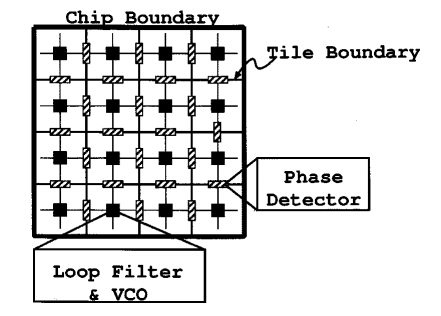
\includegraphics[scale=0.5]{../gutnik2000active}
	\caption{PLL Network Topology \cite{gutnik2000active}.}
	\label{fig:gutnik2000active}
\end{figure}

\section{ADPLL Networks}
As a PLL network is an analog circuit, its integration in a modern IC is a barrier to usage and it has not been used in any commercial designs \cite{zianbetov2013distributed}. An alternative design that is more suitable for current fabrication techniques eschews from using analog components and instead implements the network of controlled oscillators using only digital circuitry, hence the name All-Digital PLL. A 4x4 ADPLL network was designed and prototyped in 65 nm CMOS by Zianbetov and Shan in order to test the suitability of the technique as a clock distributor \cite{zianbetov2013phd,shan2014phd}. %TODO fix phd references

In this design the oscillators are coupled using digital phase comparators which attempt to measure the phase error between two oscillators with each non edge node being connected to four neighbours. Figure \ref{fig:eldar_node} shows high level detail of the architecture of both the entire clocking system and that of an individual node in the design. A digital PLL network has the additional advantages over its analog counterparts that it can benefit from advancements in digital circuit design suites, be reconfigurable and programmable and has a significantly greater immunity to perturbations inherent to its digital nature \cite{zianbetov2013phd}. This last advantage is of particular use in a digital environment, as otherwise there is potential for clock degradation resulting from switching of transistors.
\begin{figure}[h]
	\centering
	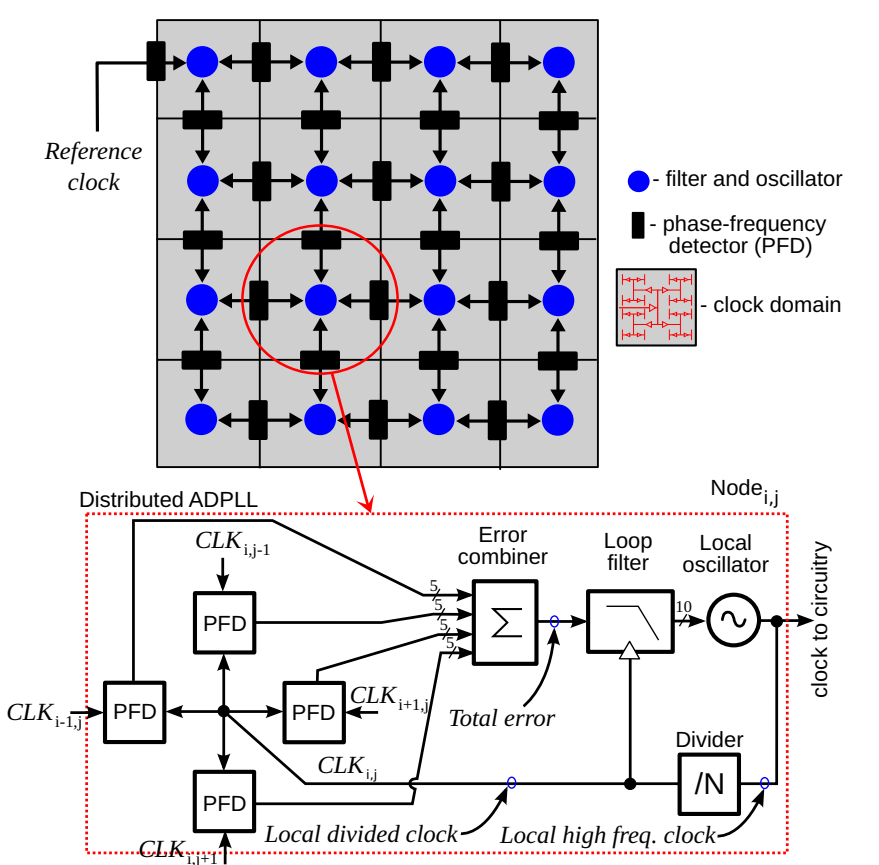
\includegraphics[scale=0.35]{../ccirc_2013_arch}
	\caption{Architecture of the ADPLL network and of a single node \cite{zianbetov2013distributed}.}
	\label{fig:eldar_node}
\end{figure}
Looking at the design of a given node it is notable that the function carried out by the Error Combiner is akin to a average, therefore as mentioned by Pratt and Nyugen, there is potential to settle in a stable ``mode'' in which the oscillators are not synchronised. In their paper, they present a method where initial start-up is performed uni-directionally and, once all nodes are close to alignment, full connectivity can be restored, however this was not viable in an analog system \cite{pratt1995distributed}. In creating an entirely digital system, Zianbetov and Shan could exploit the reconfigurability and and implement this system at start-up.

\section{ADPLL Architecture}
As indicated in Figure \ref{fig:mulkeen_pll} the three main building blocks of a conventional Phase Lock Loop are the Phase Detector, Loop Filter and Controllable Oscillator. In the All-Digital counterpart each of these traditionally analog components are replaced by their digital counterparts, necessitating quantisation in order to remain physically realisable. 
\begin{figure}[h]
	\centering
	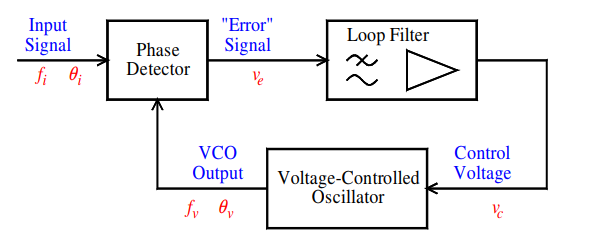
\includegraphics[scale=0.5]{mulkeen_pll}
	\caption{Block Diagram of a Phase Lock Loop, \textit{Wireless Systems Notes}, B. Mulkeen (2017).}
	\label{fig:mulkeen_pll}
\end{figure}

\subsection{Digitally Controllable Oscillator}
In a digital system there are a very limited number of voltages representable, and frequently there are only two levels, so using this to control the oscillator is not a viable strategy. Instead a fixed bit width signal is used to control the oscillator's period, selecting the number of inverters in a ring oscillator or the varactor configuration of a travelling wave oscillator \cite{chen2011rotary}. The decisions made in the design of the digitally controllable oscillator, or DCO, determine many of the other ADPLL parameters. While tuning range and centre frequency as well as linearity carry over from the analog counterpart, a DCO also has a frequency step which in combination with the bit width of the control signal determines the range over which the oscillator can be tuned. Figure \ref{fig:my_ring} illustrates a basic ring oscillator design. A ring oscillator is an inherently unstable circuit composed of an odd number of inverters where the period of oscillation is given by twice entire chain's delay. The frequency of operation can then be set by modulating the length of the chain by means of \texttt{f\_select}. The main impact of output frequency quantisation is that only frequencies which are integer multiples of the frequency step away from the centre frequency can be easily reproduced, with intermediate values only obtainable in a manner akin to Fractional-N synthesis with the control code toggling back and forth. This acts as a source of jitter in the system.
\begin{figure}[h]
	\centering
	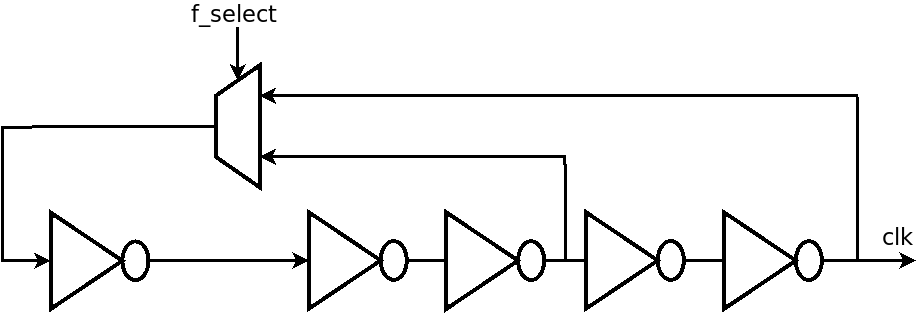
\includegraphics[scale=0.275]{../inverter_chain}
	\caption{Basic Ring/Inverter Chain Oscillator.}
	\label{fig:my_ring}
\end{figure}

\subsection{Digital Phase Detector}
Once again quantisation impacts the Phase Detector, as rather than a continuous output the phase detector in an ADPLL has a finite number of output values, thus limiting the accuracy of the phase detector. A second form of quantisation is also present, as unlike an analog system, a digital phase detector does not provide continuous data in the time domain either, instead relying on sampling. At its most basic, a digital phase comparator may only output an indication of which signal is leading, a design known as a Bang-Bang Detector, which can be constructed using a single D Flip Flop. As the output only has two levels the resultant word is only 1 bit wide and as such, limits the range over which the output frequency can be controlled. More complex designs such as that in Figure \ref{fig:shan_bb_pd}, implemented by Shan, build on this by measuring the time difference between edges of the signals using a Time-to-Digital Converter, or TDC, in his case using a tapped delay line \cite{shan2014phd}. This essentially mimics a counter and allows for a non binary form of phase measurement.

\begin{figure}[h] %TODO top
	\centering
	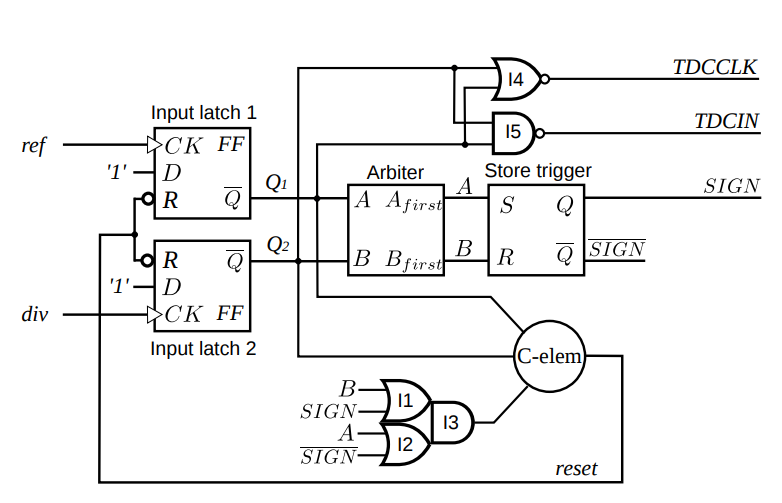
\includegraphics[scale=0.35]{../shan_bb_pd}
	\caption{Bang-bang phase/frequency detector architecture. \cite{shan2014phd}.}
	\label{fig:shan_bb_pd}
\end{figure}
\subsection{Digital Loop Filter}
\begin{figure}[h]
	\centering
	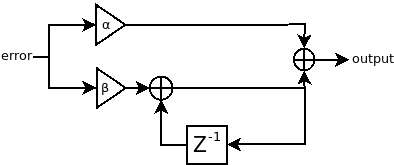
\includegraphics[scale=0.45]{../pi_simple} %TODO this diagram
	\caption{Basic PI Controller Architecture.}
	\label{fig:my_simple_pi}
\end{figure}
The loop filter in an ADPLL can be implemented as a PI controller as it is just a low pass filter, such as that in Figure \ref{fig:my_simple_pi}. In the case of an ADPLL node in a network the input of this filter is a weighted sum of two to four phase errors, each corresponding to a neighbouring node. In a digital system the proportional section is implemented by a simple multiplier, whereas the integral path is a combination of a multiplier and a delayed summation stage. The value of these gains determine the response and stability of the oscillator system. The transfer function of such a circuit is given by:
\begin{equation*}
	H(z) = \alpha + \beta\frac{1}{1-z^{-1}} = \frac{(\alpha + \beta) - \alpha z^{-1}}{1-z^{-1}}~~~\cite{shan2014phd}
\end{equation*}
It has been found by Koskin \textit{et al} (2018) that stable operation can be achieved when the integral gain, $k_i$, is less than half the proportional gain, $k_p$ \cite{koskin2018generation}. In the same study a range of values was found which would produce low jitter operation of the network. As these values are all less than one, the filter must implement fixed point arithmetic in an effort to maintain the simplicity of the clock distribution network, rather than incurring the complexity penalty of floating point calculations.

\section{My Contribution}
The planned contribution of this project is to create an FPGA based prototyping platform for the testing of network parameters and architectural variations. An FPGA as a prototyping tool for networks was previously utilised by Zianbetov and Shan as the final stage before the creation of a custom chip, as it allowed for ``a partial validation of the ASIC design, through a verification of the essential functional features of the designed clocking network'' \cite{zianbetov2013phd,shan2014phd}. They note however, that there are some fundamental differences between the two environments, in particular that the FPGA based prototype is unable to create the mixed signal circuits used in an ASIC, resulting in alternative designs being mandated for certain components such as the Time-to-Digital Converter. Similarly most commercially available FPGA boards were noted to have clock frequencies well below the gigahertz levels possible in ASIC designs. In spite of these problems, the FPGA as a prototyping solution is valuable as it allows for hardware-based testing of architectures and the simulation of non trivial circuit behaviours.

The novelty of this particular implementation is that in the case of Zianbetov and Shan only a small network was simulated on an FPGA and at a frequency close to 50 kHz, however this project will attempt to significantly increase the frequency of operation to the MHz range, as well as expanding the size of the network, from 16 oscillators to potentially 100. This is done with the aim of assisting work being undertaken by a number of researchers in UCD working on aspects of ADPLL networks who would stand to benefit from such a platform.

\chapter{Progress to Date}
The first stage of this project was the creation of an ADPLL design that would be used for the network. Due to limitations of the connections available on the FPGA evaluation board used to this point, a Digilent/Xilinx Nexys 4, outputting signals at frequencies significantly beyond 5 MHz, suffered from major degradation as the connections were not designed for such frequencies. Thus a target frequency was set at 5 MHz while this board was in use. After initial research into potential oscillator designs and what would be feasible given the constraints of the particular platform, design began with the aforementioned oscillator.

\section{Controllable Oscillator}
In my research into potential designs for numerically controllable oscillators that were viable on an FPGA I came across two main options. The first of these was the ring oscillator, constructed from an odd number of inverters strung together in a chain \cite{predraig}. In this case the frequency of operation is determined by the number of oscillators in the chain, as the delay through the individual inverters determines the half period of the signal. This period can then be modified by adding or removing inverters in a manner that maintains the odd number of total inverters. The propagation time through an individual inverter is dependant on the layout of the ring and thus this design must be used with some care.

The second option is one that I was aware of in advance of the beginning of this project. A phase accumulator makes use of the overflow property of a counter, and has a frequency determined by the width of the counter and the frequency at which it is clocked. The oscillator operates as follows: once per clock cycle the counter will increment by a number $k$ until overflow is reached at $2^n-1$ where $n$ is the bit width of the counter. By controlling the magnitude of $k$ added on each cycle of the driving clock the frequency of this oscillator can be adjusted. The most significant bit of this counter can form the clock signal, as it has an approximately 50\% duty cycle.

As it is not reliant on the clock of FPGA, the ring oscillator design is a more interesting design in the context of simulation, but the phase accumulator is significantly easier to manage due to being more easily simulatable. The decision was made to create both designs in order to keep options open.\\
The only other option I managed to come across for an oscillator on an FPGA was using Xilinx proprietary \texttt{IODELAY} blocks, which have a permanently programmable delay at runtime \cite{iodelay}. This could be coupled with an odd number of inverters in order to implement a quasi ring oscillator. However as these are IO blocks, their usage is not particularly conducive to the creation of a network of ADPLLs.

The phase accumulator was designed to have a bit width of 12, all of which could be set as the control code. As the maximum frequency of operation that had no timing violations was 258 MHz, the frequency step of this oscillator design was 62.988 kHz and before integration into an ADPLL had a frequency range from 62.988 kHz to just under half the clock frequency at 128.94 MHz. Figure \ref{fig:my_pa} details the simple construction of this oscillator.
\begin{figure}[h]
	\centering
	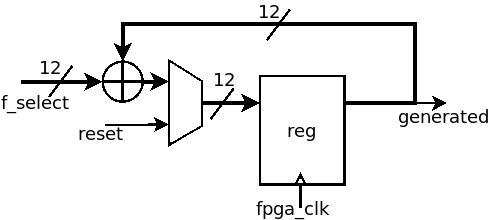
\includegraphics[scale=0.4]{../phase_accum}
	\caption{Phase Accumulator Block Diagram.}
	\label{fig:my_pa}
\end{figure}

As originally implemented for testing purposes, the inverter ring oscillator had a propagation time per inverter of 315 picoseconds, thus each inverter would add 0.63 nano seconds to the total period, and had 4 control bits. In order to obtain a 5 MHz output from this type of ring oscillator a ring of of 317 inverters is required, and to set this as the centre point of the frequency range, the total number of inverters was 325. At 5 MHz the frequency step of this design was calculated as:
\begin{align*}
T_{nom} = 200\times10^{-9}\text{ ns ,}T_{next} = 201.26\times10^{-9}\text{ ns} \\
F_{nom} = 5\times10^{6}\text{ Hz ,}F_{next} = 4.968697\times10^{-9}\text{ Hz}
\end{align*} 
\begin{equation*}
\Delta F_{RO} = 31.302\text{ kHz}
\end{equation*}
\begin{figure}[h]
	\centering
	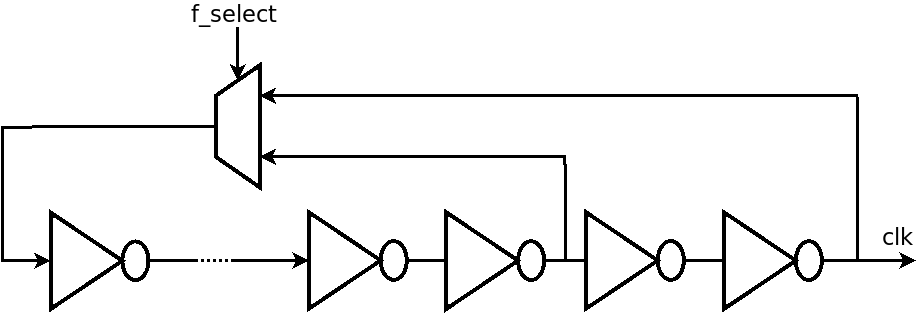
\includegraphics[scale=0.275]{../ring_osc}
	\caption{Simplified Ring Oscillator Block Diagram.}
	\label{fig:my_ring_osc}
\end{figure}
\section{Phase Detector}
Moving along the chain the next block is the phase detector, or more accurately, phase comparator. At this stage in development this block compares the oscillator's output with that of just one reference. In the future this block will be followed up with one which performs a weighted sum of all neighbouring nodes. The phase detector used in Shan's design has an arbitration circuit that is not synthesisable and an alternate design is required for use on an FPGA. The eventual design I chose has two main parts, firstly an up/down counter performs the role of the Time-to-Digital converter while also indicating the sign of the phase difference. In order to control the count and indicate the direction in which to do so, a state machine determines which edge occurs first. In order to circumvent the possibility of a metastability condition being reached, the incoming signals are synchronised to the higher frequency FPGA clock, prior to their entry into the phase detector. From there, the state machine can operate as designed, in accordance with the state transition diagram in Figure \ref{fig:my_state_machine}.
\begin{figure}[h]
	\centering
	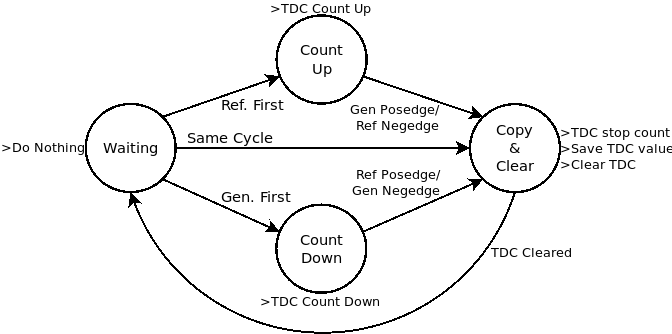
\includegraphics[scale=0.35]{../state_trans_diagram}
	\caption{Phase Detection State Machine State Transition Diagram.}
	\label{fig:my_state_machine}
\end{figure}

The state machine behaves as follows: Starting in the "Waiting" state, if the reference has a rising edge first it is said to be leading the oscillators output and the sign of the phase error is positive. Alternatively if the opposite occurs and the first rising edge is seen on the oscillator output, the phase error is given a negative sign and the TDC counts downwards. In either case, this continues until a rising edge occurs on the other signal which stops the count, updates the phase error output of the block and finally clears the counter. Between "Copy \& Clear" events, the output of the block is held constant. There is a second condition that can stop the count and that is the occurrence of a falling edge of the signal that began the count. This does however limit the rate of lock acquisition in the case where the phase difference is greater than 180$^\circ$ or where the frequency difference is significant. The operation, however, is the same as a conventional method when either locked or within a normal operating tolerance of being locked.

In order to represent both the count value and sign in one value, the counter operates in twos complement which allows the output be used directly in subsequent blocks. The counter itself has a bit width of 8, thereby having a range of -128 to 127 which at 5 MHz gives a phase resolution of:
\begin{align*}
	T_{res} &= \frac{1}{258\times 10^6} = 3.8760~ns \\
	T_{period} &= \frac{1}{5\times 10^6} = 200~ns \\
	\textrm{Ratio} &=\frac{3.8760}{200} = 0.0194 \\
	\textrm{Resolution} & = 0.0194\times 360^\circ = 6.9768^\circ
\end{align*}

\section{Loop Filter}
As with Shan's design, I used a PI controller as the loop filter, in order to align with the typical technology and to benefit from the work of members of the research team in UCD \cite{shan2014phd,koskin2018generation}.
The bit with of the filter's input is once again 8 bits, to match up with the input from the phase detector and outputs a 9 bit value in order to accommodate the summation of an 8 bit number from each of the paths. I selected $k_p = 1$ and $k_i = 0.125$ in order to align with the region of stable coefficients discovered by Eugene \cite{koskin2018generation}.
\begin{figure}[h]
	\centering
	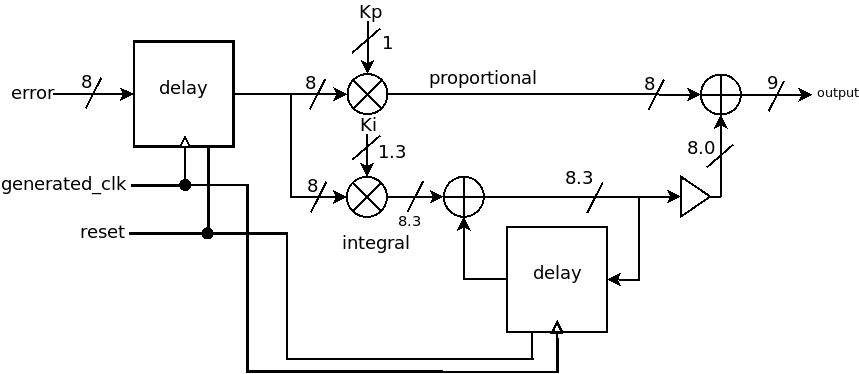
\includegraphics[scale=0.35]{../loop_filter}
	\caption{PI Loop Filter RTL diagram.}
	\label{fig:my_pi}
\end{figure}

Figure \ref{fig:my_pi} showing the RTL diagram of the filter shows the two distinct paths through the filter, the simpler of these being the proportional one. The multiplication necessitates the increased width of the path in order to preserve the accuracy of the fixed point calculations, a width which is then cut down to an 8 bit value before being added to the output of the integral branch. The proportional gain value has a fixed point width of 2.1 allowing for values from -2 to 1.5, however, in testing to this point only 1 and 0.5 have been used. The integral path is similar, with the gain having a fixed width of 1.3, a range of -1 to 0.750, and for my testing set to 0.125. After the gain is applied an accumulator with a delayed input clocked by the 258 MHz FPGA clock implements the integration. Once again the output of this path is cut back down to an 8 bit value.\\
The addition of two 8 bit values results in a 9 bit signed output from the phase detection block which is then combined with the bias to form the control code for the oscillator. As a higher control code leads to a larger frequency with the phase accumulator, this combination is done by additions, whereas for the ring oscillator the relationship is inverse as we are controlling the period, so instead subtraction is used.

\section{ADPLL}
Combining these blocks, in this case using the Phase Accumulator style oscillator, gives the ADPLL shown in Figure \ref{fig:my_adpll} on which I performed my initial testing and simulations. For ease of testing the PLL replicated the reference exactly, as this would facilitate easier testing of the lock and capture ranges of the design.
\begin{figure}[h]
	\centering
	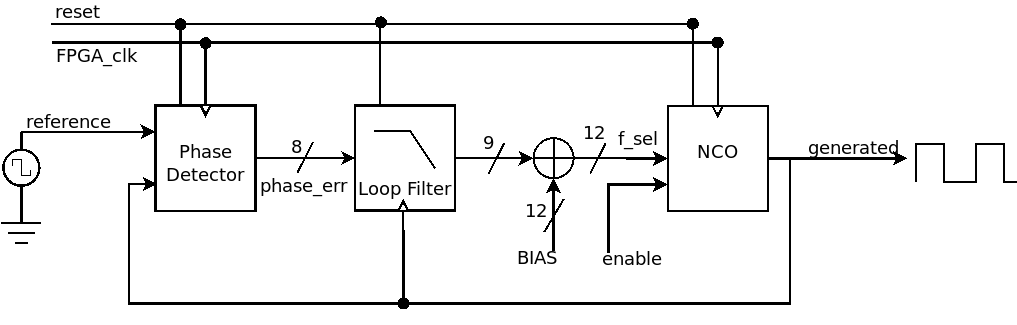
\includegraphics[scale=0.275]{../rtl}
	\caption{Phase Accumulator ADPLL RTL diagram.}
	\label{fig:my_adpll}
\end{figure}\\
Once this testing had been completed with the phase accumulator based ADPLL testing progressed to the design which implemented an inverter chain and scaling from the reference using an eight times divider. This necessitated a change in the bit width of the control signal to match the 5 bit wide signal desired, thus leading to the design in Figure \ref{fig:my_ring_adpll}.
\begin{figure}[h]
	\centering
	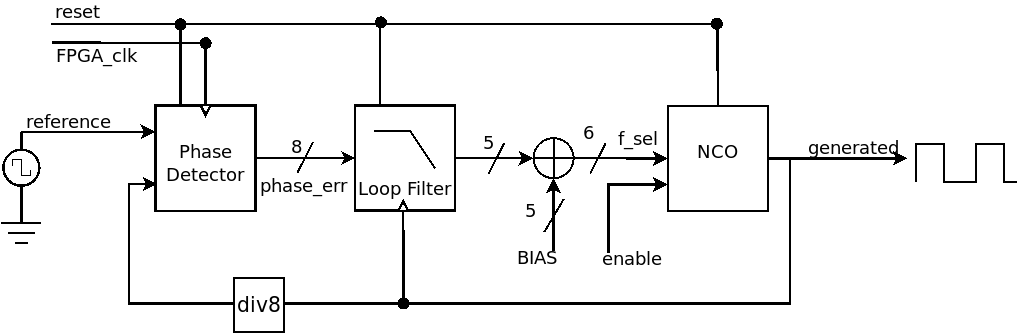
\includegraphics[scale=0.275]{../ro_rtl}
	\caption{Ring Oscillator ADPLL RTL diagram.}
	\label{fig:my_ring_adpll}
\end{figure}\\
 The Loop Filter is clocked at the generated output frequency, as this ensures it will be synchronised with the oscillator. This is important when using the inverter chain oscillator, in order to avoid metastability as the generated output clock may not be synchronised with the high frequency clock of the FPGA.


\chapter{Results}
Initially simulations were utilised to validate the behaviour of the individual blocks and of the system as a whole, while using the Phase Accumulator based design. From these simulations, I was able to test the performance of the ADPLL, while locked to a signal at 5 MHz and its behaviour during the acquisition period. A signal at 5 MHz lies close to midway between two increments of the phase accumulator and as such the oscillator must switch between two frequencies leading to the introduction of jitter. From simulations performed in Vivado locked to a signal at 5 MHz, I observed jitter of 3.491 ns, based on the differences between sequential periods, and a peak-to-peak worst case value of 9.299 ns.

Similarly, I performed simulations of the locking performance of the design, starting with a deviation of 213 KHz and observing the time taken to achieve a lock. 213 KHz represents an offset of three frequency steps, plus the difference between 5 MHz and the nearest integer frequency step. Figure \ref{fig:vivado_sim} contains the visual results of the tests, in which a repetitive pattern can be seen to begin after 20.91 $\mu$s indicating a lock as been acquired.
\begin{figure}[h]
	\centering
	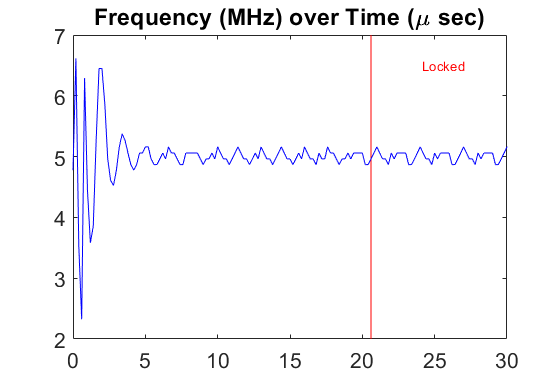
\includegraphics[scale=0.45]{../sim_locking_rect}
	\caption{Locking Dynamics Simulation.}
	\label{fig:vivado_sim}
\end{figure}

Identical tests were performed post-implementation, using a Digilent Nexys4 development board, in addition to measuring the lock and capture ranges of the design. Firstly in order to determine the baseline for jitter in the system, the oscillator was biased to 4.9761 MHz and sequential period jitter was observed to be 1.9689 ns. Connecting the remainder of the ADPLL and by varying the reference, the lock and capture ranges were found to be 4.19-12.76 MHz and 4.25-12.34 MHz respectively, when the bias point was 5 MHz. Somewhat surprisingly this is not centred on the bias point, suggesting a potential flaw in the system that needs to be addressed. A identical locking test was performed in the implemented design, Figure \ref{fig:impl}, where using the same method, a time to lock of 25.2 $\mu$s was observed. While locked jitter was better in both average period-to-period variation and in peak-to-peak, which can be attributed to the FPGA clock frequency not exactly matching that designed and as such the distance between 5 MHz and the nearest frequency step being reduced, thereby leading to less switching required to generate a 5 MHz signal.
\begin{figure}[h]
	\centering
	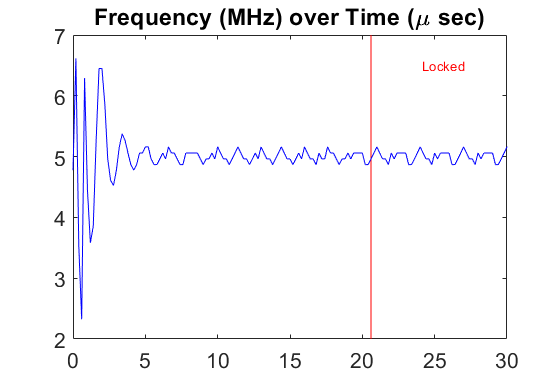
\includegraphics[scale=0.45]{../sim_locking_rect}
	\caption{Locking Dynamics Measurement.}
	\label{fig:impl}
\end{figure}

Similarly tests were carried out with the Ring Oscillator based design at a bias point of 5 MHz. 425 inverters, with 5 bit control, were used to obtain an output in the region of 5 MHz with the bias set to the midpoint which is close to 5 MHz. The expected lock range given the use of an otherwise identical design would be the entire range of 32 steps or 64 inverters which can be easily estimated:
\begin{align*}
	T_{inv} &= \frac{200\times 10^{-6}}{425-2\times 16} = 0.50891\textrm{~ns} \\
	F_{min} &= \frac{1}{(425)\times 0.50891\textrm{~ns}} = 4.623\textrm{~MHz} \\
	F_{max} &= \frac{1}{(425-2\times 32)\times 0.50891\textrm{~ns}} = 5.443\textrm{~MHz}
\end{align*}
However in testing the lock and capture ranges, both came out to be 4.86-5.15 MHz, so significantly below the estimates, which highlights an issue that requires investigation.

Testing was also carried out of the ADPLL containing a divider, in both divide by 4 and 8 modes, to examine their impact on locking behaviour. The results of this testing are displayed in Table \ref{table:b_c_perf}. The jitter in this case is rather low, as the 10 MHz target frequency lies close to an integer increment of the phase accumulator design used for this test. Lock and capture ranges are significantly more symmetrical in these configurations than at a target of 5 MHz and, as expected, there is a decrease in range with the greater division values.
\begin{figure}[h]
	\centering
	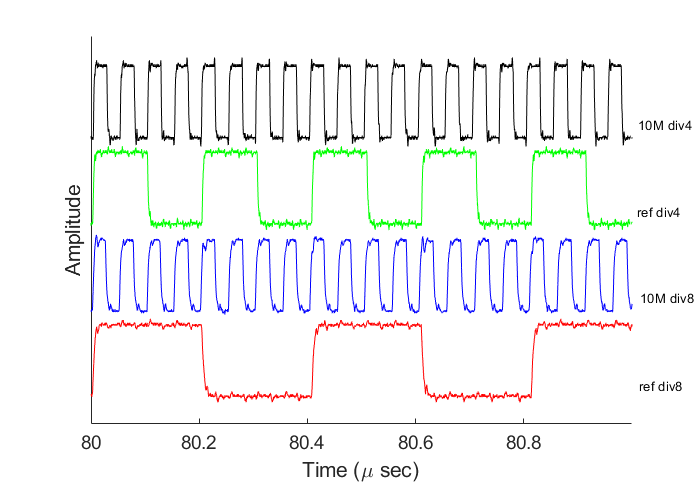
\includegraphics[scale=0.5]{../matlab/painintheass}
	\caption{Testing of ADPLLs employing div4 \& div8.}
	\label{fig:div}
\end{figure}
\begin{table}[!ht]
	\begin{center} 
		\begin{tabular}{c|c|c|c|c}           
			& Period Jitter & Peak-Peak Jitter & Lock Range & Capture Range \\
			div4 & 1.9858 ns & 6.4854 ns & 5.000-17.200 MHz & 5.620-16.700 MHz \\
			div8 & 1.5702 ns & 6.1594 ns & 5.768-15.262 MHz & 5.928-14.216 MHz \\
		\end{tabular}
		\caption{Divider Comparison.}
		\label{table:b_c_perf}
	\end{center}
\end{table}

\chapter{Future Work}
So far, all work has been done using a single phase lock loop in order to have a suitable basis for the network, and the first stage of network implementation will interlink two  of these PLLs, with one of them also receiving input from the external reference. This test will serve as both validation of the phase-coupling ability of the network as well as a test of the error summation block and the ability to lock from startup. For the sake of more realistic performance, the inverter chain ADPLL will be used ahead of the Phase Accumulator based design. With simple coupling implemented, the logical next stage is the implementation of a small network, possibly 2x2, before scaling up to a size suitable to the FPGA in use. At this point, analysis of measurement results can be undertaken and any refinements to the network can be made. Additionally, if time permits, the Phase Accumulator based design could be implemented and tested and comparisons made between both designs.

A shortcoming of the current FPGA evaluation board is the inability to input or extract signals in the multiple MHz range without significant distortion, and this will be resolved with the arrival of an FPGA more suited to extracting and importing higher frequency signals. With an ability to extract higher frequency signals for measurement and analysis purposes, the target frequency of 5 MHz can potentially be increased into the tens of MHz range.

As with the single ADPLL testing the important characteristics to look out for will be the lock and capture ranges of the network which should mirror that of the ADPLLs used in it's construction. Similarly the jitter of a number of clocks across the network will be examined in order, and any skew between the PLL outputs investigated. Also of interest will be the initial locking behaviour, in particular how quickly the network can be brought up from ``cold''.

\newpage
\bibliography{bib} 
\bibliographystyle{IEEEtran}

\end{document}
